\documentclass[12pt, titlepage]{article}

\usepackage{fullpage}
\usepackage[round]{natbib}
\usepackage{multirow}
\usepackage{booktabs}
\usepackage{tabularx}
\usepackage{graphicx}
\usepackage{float}
\usepackage{hyperref}
\hypersetup{
    colorlinks,
    citecolor=blue,
    filecolor=black,
    linkcolor=red,
    urlcolor=blue
}

\input{../../Comments}
%% Common Parts

\newcommand{\progname}{Software Engineering} % PUT YOUR PROGRAM NAME HERE
\newcommand{\authname}{Team 8, AlgoCatan
\\ Jake Read
\\ Rebecca Di Filippo
\\ Matthew Cheung
\\ Sunny Yao} % AUTHOR NAMES

\usepackage{hyperref}
    \hypersetup{colorlinks=true, linkcolor=blue, citecolor=blue, filecolor=blue,
                urlcolor=blue, unicode=false}
    \urlstyle{same}
                                


\newcounter{acnum}
\newcommand{\actheacnum}{AC\theacnum}
\newcommand{\acref}[1]{AC\ref{#1}}

\newcounter{ucnum}
\newcommand{\uctheucnum}{UC\theucnum}
\newcommand{\uref}[1]{UC\ref{#1}}

\newcounter{mnum}
\newcommand{\mthemnum}{M\themnum}
\newcommand{\mref}[1]{\hyperref[sec:#1]{M\ref*{#1}}}

\begin{document}

\title{Module Guide for \progname{}}
\author{\authname}
\date{January 19th, 2026}

\maketitle

\pagenumbering{roman}

\section{Revision History}

\begin{tabularx}{\textwidth}{p{3cm}p{2cm}X}
\toprule {\bf Date} & {\bf Version} & {\bf Notes}\\
\midrule
11/13/2025 & 1.0 & Rev -1\\
01/14/2026 & 1.1 & Rev 0\\
04/06/2026 & 1.2 & Final Doc Review\\
\bottomrule
\end{tabularx}

\newpage

\section{Reference Material}

This section records information for easy reference.

\subsection{Abbreviations and Acronyms}

\renewcommand{\arraystretch}{1.2}
\begin{tabular}{l l}
  \toprule
  \textbf{symbol} & \textbf{description}\\
  \midrule
  AC & Anticipated Change\\
  AI & Artificial Intelligence \\
  LLM & Large Language Model \\
  CV & Computer Vision \\
  DAG & Directed Acyclic Graph \\
  FR & Functional Requirement \\
  M & Module \\
  MG & Module Guide \\
  NFR & Non-Functional Requirement \\
  OS & Operating System \\
  R & Requirement\\
  RL & Reinforcement Learning \\
  SRS & Software Requirements Specification\\
  UC & Unlikely Change \\
  UI & User Interface \\
  VnV & Verification and Validation \\
  \bottomrule
\end{tabular}\\

\newpage

\tableofcontents

\listoftables

\listoffigures

\newpage

\pagenumbering{arabic}

\section{Introduction}

Decomposing a system into modules is a commonly accepted approach to developing software.
A module is a work assignment for a programmer or programming team~\citep{ParnasEtAl1984}.
We advocate a decomposition based on the principle of information hiding~\citep{Parnas1972a}.
This principle supports design for change, because the ``secrets'' that each module hides represent likely future changes.
Our design follows the rules layed out by \citet{ParnasEtAl1984}, as follows:
\begin{itemize}
\item System details that are likely to change independently should be the secrets of separate modules.
\item Each data structure is implemented in only one module.
\item Any other program that requires information stored in a module's data structures must obtain it by calling access programs belonging to that module.
\end{itemize}

After completing the first stage of the design, the Software Requirements
Specification (SRS), the Module Guide (MG) is developed~\citep{ParnasEtAl1984}.
The MG specifies the modular structure of the system and is intended to allow both designers and maintainers to easily identify the parts of the software.
The rest of the document is organized as follows. Section
\ref{SecChange} lists the anticipated and unlikely changes of the software requirements.
Section \ref{SecMH} summarizes the module decomposition that was constructed according to the likely changes.
Section \ref{SecConnection} specifies the connections between the software requirements and the
modules.
Section \ref{SecMD} gives a detailed description of the modules.
Section \ref{SecTM} includes two traceability matrices.
One checks the completeness of the design against the requirements provided in the SRS\@.
The other shows the relation between anticipated changes and the modules.
Section
\ref{SecUse} describes the use relation between modules.

\section{Anticipated and Unlikely Changes} \label{SecChange}

This section lists possible changes to the system.
According to the likeliness of the change, the possible changes are classified into two categories.
Anticipated changes are listed in Section \ref{SecAchange}, and unlikely changes are listed in Section \ref{SecUchange}.

\subsection{Anticipated Changes} \label{SecAchange}

Anticipated changes are the source of the information that is to be hidden inside the modules.
Ideally, changing one of the anticipated changes will only require changing the one module that hides the associated decision.

\begin{description}
\item[\refstepcounter{acnum} \actheacnum \label{acAIModel}:] The specific architecture, heuristics, and reward functions of the RL agent.
These will be iterated on constantly to improve performance.
\item[\refstepcounter{acnum} \actheacnum \label{acCVModel}:] The specific CV algorithm or model (e.g., YOLOv9 vs.
OpenCV) used for board state detection (Deferred).
This may be changed to improve accuracy or adapt to different lighting conditions.
\item[\refstepcounter{acnum} \actheacnum \label{acUI}:] The layout and design of the User Interface.
This will likely change based on user feedback to improve usability.
\item[\refstepcounter{acnum} \actheacnum \label{acSimulator}:] The underlying Catan simulator (Catanatron).
This is an external library that may be updated or replaced.
\item[\refstepcounter{acnum} \actheacnum \label{acDatabase}:] The specific schema or technology (e.g., SQL vs NoSQL) for the Game State Database, as post-game analysis needs may evolve.
\item[\refstepcounter{acnum} \actheacnum \label{acComm}:] The communication protocol (e.g., 0MQ) used by the Image Queue.
This might be swapped for another low-latency middleware like WebSockets (Deferred).
\end{description}

\subsection{Unlikely Changes} \label{SecUchange}

The module design should be as general as possible.
However, fixing some design decisions at the system architecture stage can simplify the software design.
It is not intended that these decisions will be changed.

\begin{description}
\item[\refstepcounter{ucnum} \uctheucnum \label{ucGameRules}:] The fundamental rules of the standard Settlers of Catan base game.
The project is not intended to support expansions.
\item[\refstepcounter{ucnum} \uctheucnum \label{ucArchitecture}:] The core architectural decomposition.
The system will always require separate components for vision, state management, AI, and a user interface.
\item[\refstepcounter{ucnum} \uctheucnum \label{ucTechStack}:] The primary technology stack choices of Python for the backend/AI and JavaScript/React for the frontend.
\item[\refstepcounter{ucnum} \uctheucnum \label{ucInputSource}:] The fundamental premise of reading from a physical game board via a camera, as opposed to being a purely digital application (Deferred).
\end{description}


\section{Module Hierarchy} \label{SecMH}

This section provides an overview of the module design.
Modules are summarized in a hierarchy decomposed by secrets in Table \ref{TblMH}.
The modules listed below, which are leaves in the hierarchy tree, are the modules that will actually be implemented.

\begin{description}
\item [\refstepcounter{mnum} \mthemnum \label{mHH}:] Hardware-Hiding Module (OS) (Deferred)
\item [\refstepcounter{mnum} \mthemnum \label{mCV}:] Computer Vision Model (Deferred)
\item [\refstepcounter{mnum} \mthemnum \label{mUI}:] User Interface
\item [\refstepcounter{mnum} \mthemnum \label{mState}:] Game State Manager
\item [\refstepcounter{mnum} \mthemnum \label{mEnv}:] Training Pipeline
\item [\refstepcounter{mnum} \mthemnum \label{mAI}:] AI Model
\item [\refstepcounter{mnum} \mthemnum \label{mDB}:] Game State Database
\item [\refstepcounter{mnum} \mthemnum \label{mQueue}:] Backend API Server
\item [\refstepcounter{mnum} \mthemnum \label{mLeague}:] Elo League System
\item [\refstepcounter{mnum} \mthemnum \label{mCurriculum}:] Curriculum Learning Manager
\item [\refstepcounter{mnum} \mthemnum \label{mExplain}:] Explanation Pipeline
\end{description}

\begin{table}[h!]
\centering
\caption{Module Hierarchy}
\label{TblMH}
\begin{tabular}{p{0.3\textwidth} p{0.6\textwidth}}
\toprule
\textbf{Level 1} & \textbf{Level 2}\\
\midrule

\multirow{2}{0.3\textwidth}{Hardware-Hiding Module}
& \mref{mHH}: Hardware-Hiding Module (OS) \\
& \mref{mCV}: Computer Vision Model \\
\midrule

\multirow{3}{0.3\textwidth}{Behaviour-Hiding Module}
& \mref{mUI}: User Interface \\
& \mref{mState}: Game State Manager \\
& \mref{mEnv}: Training Pipeline \\
\midrule

\multirow{6}{0.3\textwidth}{Software Decision Module}
& \mref{mAI}: AI Model \\
& \mref{mDB}: Game State Database \\
& \mref{mQueue}: Backend API Server \\
& \mref{mLeague}: Elo League System \\
& \mref{mCurriculum}: Curriculum Learning Manager \\
& \mref{mExplain}: Explanation Pipeline \\
\bottomrule
\end{tabular}
\end{table}



\section{Connection Between Requirements and Design} \label{SecConnection}

The design of the system is intended to satisfy the requirements developed in
the SRS. The following key design decisions were made to address specific requirements:

\begin{itemize}
    \item \textbf{Training Pipeline (\mref{mEnv}):} To satisfy FR.S.2.x and support FR.Sa.12, a dedicated training pipeline coordinates self-play, reward collection, evaluation, checkpointing, and integration with both curriculum phases and league-based opponent selection.

    \item \textbf{AI Model (\mref{mAI}):} To satisfy FR.S.3.1--FR.S.3.5, the AI model module encapsulates inference logic, model weights, and move selection behaviour, allowing model versions to be swapped independently of the rest of the system.

    \item \textbf{Elo League System (\mref{mLeague}):} To satisfy FR.S.3.6--FR.S.3.10, a dedicated league module maintains ratings for trained snapshots and baseline bots, supports opponent selection, and manages pruning/storage policies.

    \item \textbf{Curriculum Learning Manager (\mref{mCurriculum}):} To satisfy FR.S.3.12--FR.S.3.16, curriculum phase definitions and advancement rules are isolated in their own module so that training complexity can evolve without changing unrelated system logic.

    \item \textbf{User Interface (\mref{mUI}):} To satisfy FR.S.4.x and NFR.S.2, the web frontend is isolated as its own module, enabling independent iteration of gameplay presentation, replay views, bot selection, and explanation display.

    \item \textbf{Game State Database (\mref{mDB}):} To satisfy FR.S.5.x and NFR.S.5, a dedicated database module manages persistent storage for game history, replay data, model metadata, and league-related records.

    \item \textbf{Backend API Server (\mref{mQueue}):} To satisfy FR.S.6.x, NFR.S.1, and NFR.S.6, a dedicated backend communication layer handles requests between the frontend and backend modules, including gameplay, replay, bot selection, and explanation requests.

    \item \textbf{Game State Manager (\mref{mState}):} To satisfy FR.S.7.x and FR.Sa.2--FR.Sa.3, the authoritative game state and move validation logic are encapsulated in a separate module to preserve consistency across gameplay, replay, and explanation workflows.

    \item \textbf{Explanation Pipeline (\mref{mExplain}):} To satisfy FR.S.8.x, a dedicated explanation module formats move/state context, communicates with the external LLM service, and returns user-facing natural-language explanations independently of the core AI inference module.

    \item \textbf{Computer Vision Module (\mref{mCV}):} The CV module is retained only for deferred future scope, preserving traceability to FR.S.1.x and related safety requirements without affecting the present web-based architecture.

    \item \textbf{Hardware-Hiding Module (\mref{mHH}):} This module is also deferred, as the current design focuses on a purely digital implementation. However, its inclusion in the hierarchy allows for future expansion to support physical board input without major architectural changes.
\end{itemize}



\section{Module Decomposition} \label{SecMD}

Modules are decomposed according to the principle of ``information hiding''
proposed by \citet{ParnasEtAl1984}.
The \emph{Secrets} field in a module
decomposition is a brief statement of the design decision hidden by the
module.
The \emph{Services} field specifies \emph{what} the module will do
without documenting \emph{how} to do it.

\subsection{Hardware Hiding Modules}

\subsubsection{Hardware-Hiding Module (\mref{mHH})} \label{sec:mHH}
\begin{description}
\item[Secrets:] The data structures and algorithms used to implement the underlying virtual hardware and platform services.
Camera-specific device interaction is only relevant if the deferred CV path is later implemented.
\item[Services:] Serves as virtual hardware used by the rest of the system.
This module provides the interface between the operating system/platform and the software.
\item[Implemented By:] OS
\end{description}

\subsubsection{Computer Vision Model (\mref{mCV})} \label{sec:mCV}
\begin{description}
\item[Secrets:] The specific algorithms, libraries (e.g., OpenCV, YOLOv9), and trained models used to interpret a raw video/image feed and detect the physical board layout, pieces, and player actions.
Hides the complexity of calibration and error correction.
\item[Services:] Provides access programs to process camera input, detect board elements, and translate visual features into a structured digital representation of the game state.
Provides diagnostic feedback on detection confidence.
This module is deferred and not part of the current implementation.
\item[Implemented By:] Python using OpenCV/YOLOv9-based computer vision tooling, trained models, and supporting scripts within \progname{}
\end{description}

\subsection{Behaviour-Hiding Module}
\begin{description}
\item[Secrets:] The contents of the required behaviours.
\item[Services:] Includes programs that provide externally visible behaviour of
the system as specified in the SRS.
This module serves as a communication layer between the user-facing functionality and the underlying software decision modules.
\item[Implemented By:] --
\end{description}

\subsubsection{User Interface (\mref{mUI})} \label{sec:mUI}
\begin{description}
\item[Secrets:] The specific frontend framework, state presentation logic, UI/UX choices, and replay/explanation interaction patterns used to render the system.
Hides the details of DOM manipulation, component composition, and client-side event handling.
\item[Services:] Provides an interactive visualization of the \emph{Catan} board and current game state.
Allows users to play games, view replays, select opponents, and request/display move explanations.
\item[Implemented By:] React/JavaScript frontend.
\end{description}

\subsubsection{Game State Manager (\mref{mState})} \label{sec:mState}
\begin{description}
\item[Secrets:] The internal data structures and logic used to represent the authoritative game state and enforce the official \emph{Catan} ruleset.
Hides synchronization and validation logic across gameplay and replay.
\item[Services:] Maintains the single source of truth for the current game state.
Tracks player assets, turn data, and legal actions.
Provides access programs to update, query, and validate game states and moves.
\item[Implemented By:] Integration and Python-based modification of the open-source Catanatron simulator.
\end{description}

\subsubsection{Training Pipeline (\mref{mEnv})} \label{sec:mEnv}
\begin{description}
\item[Secrets:] The orchestration logic for training runs, including simulator integration, checkpointing, evaluation scheduling, metric collection, and coordination with curriculum and league modules.
\item[Services:] Runs and manages AI training workflows.
Coordinates self-play, reward collection, evaluation, and model checkpoint generation.
Provides access programs for launching and monitoring training runs.
\item[Implemented By:] Python training scripts and orchestration code.
\end{description}

\subsection{Software Decision Module}
\begin{description}
\item[Secrets:] The design decision based on mathematical theorems, physical
facts, or programming considerations.
The secrets of this module are
\emph{not} described in the SRS.
\item[Services:] Includes data structures and algorithms used in the system that
do not provide direct interaction with the user.
\item[Implemented By:] --
\end{description}

\subsubsection{AI Model (\mref{mAI})} \label{sec:mAI}
\begin{description}
\item[Secrets:] The specific DRL model architecture, heuristics, feature encoding, and trained weights used to determine actions.
Hides the mathematical formulation and implementation details of policy/value inference.
\item[Services:] Analyzes a given game state and produces valid actions or action evaluations.
Provides access programs for move inference and model version loading.
\item[Implemented By:] PPO-based DRL model implementation.
\end{description}

\subsubsection{Game State Database (\mref{mDB})} \label{sec:mDB}
\begin{description}
\item[Secrets:] The specific database technology, schema, indexing strategy, and persistence logic used to store and retrieve game history, replay data, model metadata, and league-related records.
\item[Services:] Stores and maintains complete and consistent records of game states, match results, replay data, and model metadata.
Provides access programs for efficient read/write operations and structured access to historical data.
\item[Implemented By:] PostgreSQL database layer.
\end{description}

\subsubsection{Backend API Server (\mref{mQueue})} \label{sec:mQueue}
\begin{description}
\item[Secrets:] The specific API framework, endpoint structure, serialization format, request/response contracts, and error-handling logic used for frontend/backend communication.
\item[Services:] Enables reliable communication between the User Interface and backend modules.
Provides access programs for gameplay, replay, bot selection, persistence, and explanation requests.
\item[Implemented By:] Python backend API layer.
\end{description}

\subsubsection{Elo League System (\mref{mLeague})} \label{sec:mLeague}
\begin{description}
\item[Secrets:] The Elo update rules, baseline sampling policy, snapshot retention strategy, and league pruning logic used to manage model strength estimation and opponent selection.
\item[Services:] Maintains ratings for trained model snapshots and baseline bots.
Provides access programs to register league members, update ratings, expose available opponents, and select opponents for training or gameplay.
\item[Implemented By:] Python-based software engineering.
\end{description}

\subsubsection{Curriculum Learning Manager (\mref{mCurriculum})} \label{sec:mCurriculum}
\begin{description}
\item[Secrets:] The curriculum phase definitions, advancement thresholds, cycling rules, and rule-variation configuration used to control training complexity.
\item[Services:] Defines and manages curriculum phases for training.
Provides access programs to determine the active phase, evaluate advancement conditions, and log phase transitions.
\item[Implemented By:] Python-based software engineering.
\end{description}

\subsubsection{Explanation Pipeline (\mref{mExplain})} \label{sec:mExplain}
\begin{description}
\item[Secrets:] The prompt construction logic, context-packet format, provider-specific LLM integration, and response validation/filtering used to generate natural-language move explanations.
\item[Services:] Collects the relevant game-state and move context for an explanation request.
Formats requests for the external LLM service and returns user-facing natural-language explanations or clear failure responses.
\item[Implemented By:] Python-based backend explanation services with external LLM API integration
\end{description}

\newpage
\section{Traceability Matrix} \label{SecTM}

This section shows two traceability matrices: between the modules and the
requirements and between the modules and the anticipated changes.


\begin{table}[H]
\centering
\caption{Trace Between Requirements and Modules}
\label{TblRT}
\begin{tabularx}{\textwidth}{|l|X|}
\hline
\textbf{Requirement(s)} & \textbf{Modules}\\
\hline
FR.S.1.x (Computer Vision Model, Deferred) & \mref{mCV} \\
\hline
FR.S.2.x (Training Pipeline) & \mref{mEnv}, \mref{mLeague}, \mref{mCurriculum} \\
\hline
FR.S.3.1--FR.S.3.5 (AI Model) & \mref{mAI} \\
\hline
FR.S.3.6--FR.S.3.10 (Elo League System) & \mref{mLeague}, \mref{mDB} \\
\hline
FR.S.3.12--FR.S.3.16 (Curriculum Learning Manager) & \mref{mCurriculum}, \mref{mEnv} \\
\hline
FR.S.4.x (User Interface) & \mref{mUI}, \mref{mLeague}, \mref{mExplain} \\
\hline
FR.S.5.x (Game State DB) & \mref{mDB} \\
\hline
FR.S.6.x (Backend API Server) & \mref{mQueue} \\
\hline
FR.S.7.x (Game State Manager) & \mref{mState} \\
\hline
FR.S.8.x, FR.Sa.13 (Explanation Pipeline) & \mref{mExplain}, \mref{mQueue} \\
\hline
NFR.S.1 (Scalability) & \mref{mAI}, \mref{mDB}, \mref{mQueue}, \mref{mExplain} \\
\hline
NFR.S.2 (Usability) & \mref{mUI}, \mref{mExplain} \\
\hline
NFR.S.3 (Maintainability) & \mref{mAI}, \mref{mCV}, \mref{mState}, \mref{mUI}, \mref{mEnv}, \mref{mQueue}, \mref{mLeague}, \mref{mCurriculum}, \mref{mExplain} \\
\hline
NFR.S.4 (Installability) & \mref{mHH}, \mref{mQueue}, \mref{mUI} \\
\hline
NFR.S.5 (Data Integrity) & \mref{mDB}, \mref{mState}, \mref{mQueue} \\
\hline
NFR.S.6 (Availability) & \mref{mQueue}, \mref{mDB}, \mref{mExplain} \\
\hline
FR.Sa.1, FR.Sa.8, FR.Sa.11 (Deferred CV Safety) & \mref{mCV}, \mref{mUI} \\
\hline
FR.Sa.2 (State Resynchronization) & \mref{mState}, \mref{mUI} \\
\hline
FR.Sa.3 (AI Validation) & \mref{mState}, \mref{mAI} \\
\hline
FR.Sa.4 (Graceful Failure Messaging) & \mref{mUI}, \mref{mQueue}, \mref{mExplain} \\
\hline
FR.Sa.5 (DB Safety) & \mref{mDB} \\
\hline
FR.Sa.6, NFR.Sa.2 (Connection Safety) & \mref{mQueue} \\
\hline
FR.Sa.7 (Suggestion Visibility) & \mref{mUI} \\
\hline
FR.Sa.9 (Incomplete Data Warning) & \mref{mUI}, \mref{mExplain}, \mref{mCV} \\
\hline
FR.Sa.10 (AI Rollback) & \mref{mAI}, \mref{mLeague} \\
\hline
FR.Sa.12, 14, 15 (Training Validation) & \mref{mEnv}, \mref{mLeague}, \mref{mCurriculum} \\
\hline
\end{tabularx}
\end{table}



\begin{table}[H]
\centering
\caption{Trace Between Anticipated Changes and Modules}
\label{TblACT}
\begin{tabular}{|l|l|}
\hline
\textbf{Anticipated Change (AC)} & \textbf{Modules}\\
\hline
\acref{acAIModel} & \mref{mAI} \\
\hline
\acref{acCVModel} & \mref{mCV} \\
\hline
\acref{acUI} & \mref{mUI} \\
\hline
\acref{acSimulator} & \mref{mEnv} \\
\hline
\acref{acDatabase} & \mref{mDB} \\
\hline
\acref{acComm} & \mref{mQueue} \\
\hline
\end{tabular}
\end{table}

\begin{table}[H]
\centering
\caption{Trace Between Unlikely Changes and Modules}
\label{TblUCT}
\begin{tabular}{|l|l|}
\hline
\textbf{Unlikely Change (UC)} & \textbf{Modules}\\
\hline
\uref{ucGameRules} & \mref{mEnv} \\
\hline
\end{tabular}
\end{table}

\section{Use Hierarchy Between Modules} \label{SecUse}

In this section, the uses hierarchy between modules is provided.
Module A uses a module B if the correct execution of A depends upon the availability of a correct implementation of B.

For the current system, runtime dependencies are centered around the Backend API Server (\mref{mQueue}),
while training-side dependencies are centered around the Training Pipeline (\mref{mEnv}).

At runtime, the User Interface (\mref{mUI}) depends on the Backend API Server (\mref{mQueue}),
which in turn depends on the Game State Manager (\mref{mState}), Game State Database (\mref{mDB}),
AI Model (\mref{mAI}), Elo League System (\mref{mLeague}), and Explanation Pipeline (\mref{mExplain})
depending on the request type.

\begin{figure}[H]
\centering
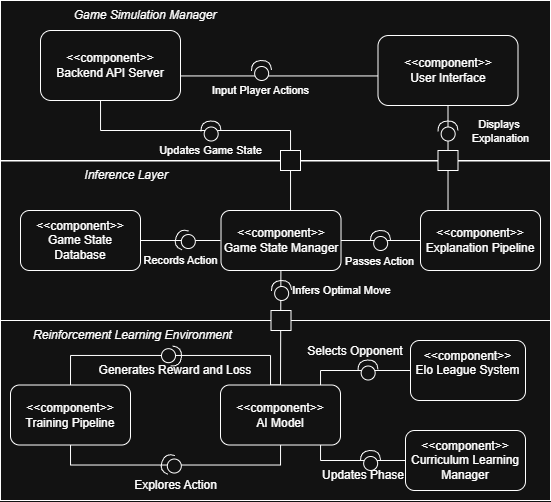
\includegraphics[width=\textwidth]{Component_Diagram_final}
\caption{Component diagram showing use hierarchy among modules.}
\label{FigUH}
\end{figure}

\section{User Interfaces}

The detailed design of the User Interface (\mref{mUI}) will be designed in stages, and updated following user feedback.
As such, the specific UI design is not included in this document.
(The usability testing doc in the extras folder covers the iteration process for the UI design in more detail.)
The design will focus on satisfying NFR.S.2 (Usability) and the specific UI-related safety requirements (e.g., FR.Sa.1, FR.Sa.7).

\section{Design of Communication Protocols}

The system's runtime modules communicate primarily through the Backend API Server (\mref{mQueue}).
In the implemented system, this communication is based on REST-style HTTP requests carrying JSON payloads.

The frontend uses the backend base URL specified by the \texttt{CTRON\_API\_URL} environment variable,
defaulting to \texttt{http://localhost:5001} in local development.
The backend is implemented as a Flask application with CORS enabled, and its API routes are exposed through
a blueprint mounted under the \texttt{/api} prefix.

\subsection*{Runtime API Contracts}

\begin{itemize}
    \item \texttt{POST /api/analytics/start} \\
    Called by the frontend when a user starts interacting with the application.
    Logs a homepage/game-start analytics event and returns whether the event was recorded successfully.

    \item \texttt{GET /api/admin/user-starts?limit=<n>} \\
    Used by the admin page to retrieve recently logged user-start events.
    Returns a JSON array of rows containing \texttt{id}, \texttt{ip}, and \texttt{timestamp} fields.

    \item \texttt{GET /api/bots} \\
    Used by the bot-selection pages to retrieve available opponents.
    Returns bot metadata including identifiers, display names, Elo values, and backend player keys.

    \item \texttt{POST /api/games} \\
    Creates a new game session.
    The request body includes a \texttt{players} array and may also include optional configuration such as
    \texttt{map\_template}, \texttt{discard\_limit}, \texttt{vps\_to\_win}, \texttt{friendly\_robber}, and \texttt{familiarity}.
    The response returns a generated \texttt{game\_id}.

    \item \texttt{GET /api/games/\{gameId\}/states/\{stateIndex\}} \\
    Retrieves a serialized game state for the specified game and state index.
    The special value \texttt{latest} may be used instead of a numeric state index.

    \item \texttt{POST /api/games/\{gameId\}/actions} \\
    Advances the game by one action.
    If the request body is empty, the backend treats the request as a bot turn.
    If the request body contains an action object, the backend parses and executes the supplied human action.

    \item \texttt{GET /api/games/\{gameId\}/states/\{stateIndex\}/mcts-analysis} \\
    Requests analysis data for a particular stored state.
    Returns JSON containing a success flag, win-probability estimates, and the analyzed state index.

    \item \texttt{GET /api/games/\{gameId\}/explain/\{moveIndex\}} \\
    Requests an LLM explanation for a specific move in the selected game.
    Returns JSON containing the queried move index and the generated natural-language explanation.
\end{itemize}

\subsection*{Frontend Usage of the Protocol}

The User Interface (\mref{mUI}) communicates with the Backend API Server (\mref{mQueue}) through a typed
frontend API client.
Bot-selection screens request available bots and create configured games.
Gameplay and replay screens request serialized game states, submit actions, request MCTS analysis,
and request move explanations when the user selects ``Explain Move''.

\subsection*{Internal Backend Coordination}

Behind these HTTP endpoints, the Backend API Server coordinates with the Game State Manager (\mref{mState}),
Game State Database (\mref{mDB}), AI Model (\mref{mAI}), Elo League System (\mref{mLeague}),
and Explanation Pipeline (\mref{mExplain}) through direct Python calls and shared backend objects.
These internal interactions are implementation-level module uses rather than separate externally visible network protocols.


\section{Timeline}

The schedule of tasks for the implementation of Revision 0 is detailed below.
This timeline ensures that the core components are implemented and integrated by the Rev 0 deadline of February 2, 2026.
Tasks are assigned to specific team members corresponding to the modules defined in this document.
Note that some modules are absent from the table, as they were added post-revision 0, or were deferred at the time of writing.

\begin{table}[H]
\centering
\caption{Implementation Timeline for Revision 0}
\label{TblTimeline}
\begin{tabularx}{\textwidth}{|l|X|l|l|}
\toprule
\textbf{Module} & \textbf{Task Description} & \textbf{Assignee} & \textbf{Due Date} \\
\midrule
\mref{mAI} & \textbf{Advanced Action Masking}: Refine gym wrappers to strictly filter invalid moves to reduce effective state space. & Jake & Jan 18 \\
\hline
\mref{mAI} & \textbf{Heuristic-Guided Exploration}: Integrate human logic heuristics to guide agent exploration during early training. & Rebecca & Jan 22 \\
\hline
\mref{mAI} & \textbf{Reward Shaping v2}: Analyze v1 logs to fix behavior loops (e.g., road spamming) and implement complex reward signals. & Jake, Rebecca & Jan 24 \\
\hline
\mref{mCV} & \textbf{Exploratory Feasibility Study}: Standalone research script to test if board state can be reliably detected from static images. & Matthew & Jan 28 \\
\hline
\mref{mUI} & \textbf{Agent Visualization}: Adapt CLI visualizer or lightweight web view to display agent metrics (Confidence/Win \%) live. & Sunny & Jan 30 \\
\hline
\mref{mEnv} & \textbf{Benchmarking Suite}: Setup automated evaluation against baseline bots to generate win-rate graphs. & Sunny & Jan 31 \\
\hline
All & \textbf{Rev 0 Training Run}: Execute final 48+ hour training session using finalized v2 rewards and masks. & Team & Feb 1 \\
\hline
All & \textbf{Rev 0 Verification}: Analyze final model to ensure it beats Random Baseline $>$95\% and competes with heuristic bots. & Team & Feb 2 \\
\bottomrule
\end{tabularx}
\end{table}

\bibliographystyle{plainnat}

%\bibliography{../../../refs/References}

\newpage{}

\end{document}